\chapter{系统硬件设计}

本章在总体架构和器件选型基础上，给出各硬件子模块的电路设计思路与连接关系，明确系统从器件到整机的实现路径。

\section{单片机控制核心电路}

主控电路包含最小系统、电源管理、时钟与下载调试接口。设计中重点保证供电稳定、复位可靠与信号完整，以提高系统连续运行能力。

瞄准模块以STM32H743核心板为中心，外围扩展RS485电机总线接口、HiPNUC IMU串口接口和视觉串口接口。电路原理图如图\ref{fig:aim-schematic}所示。

\begin{figure}[H]
\centering
\subfigure[瞄准模块电路原理图\label{fig:aim-schematic}]{{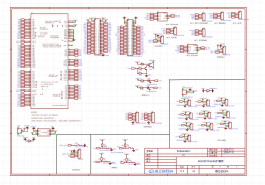
\includegraphics[width=0.8\textwidth]{images/chapters/fig-aim-schematic.png}}}
\label{fig:aim-board}
\end{figure}

原理图中，STM32H7通过若干GPIO扩展了电机RS485收发器、IMU UART接口及指示LED等外围器件；PCB布局充分考虑了高频信号与电源回路的分离，减少干扰。图\ref{fig:stm32h7-board}为所用STM32H743核心板实物图，芯片封装为LQFP144，板载Winbond W9825G6KH-6I外扩SDRAM，具备充足的运行内存供RT-Thread操作系统及多线程控制任务使用。

\begin{figure}[H]
\centering
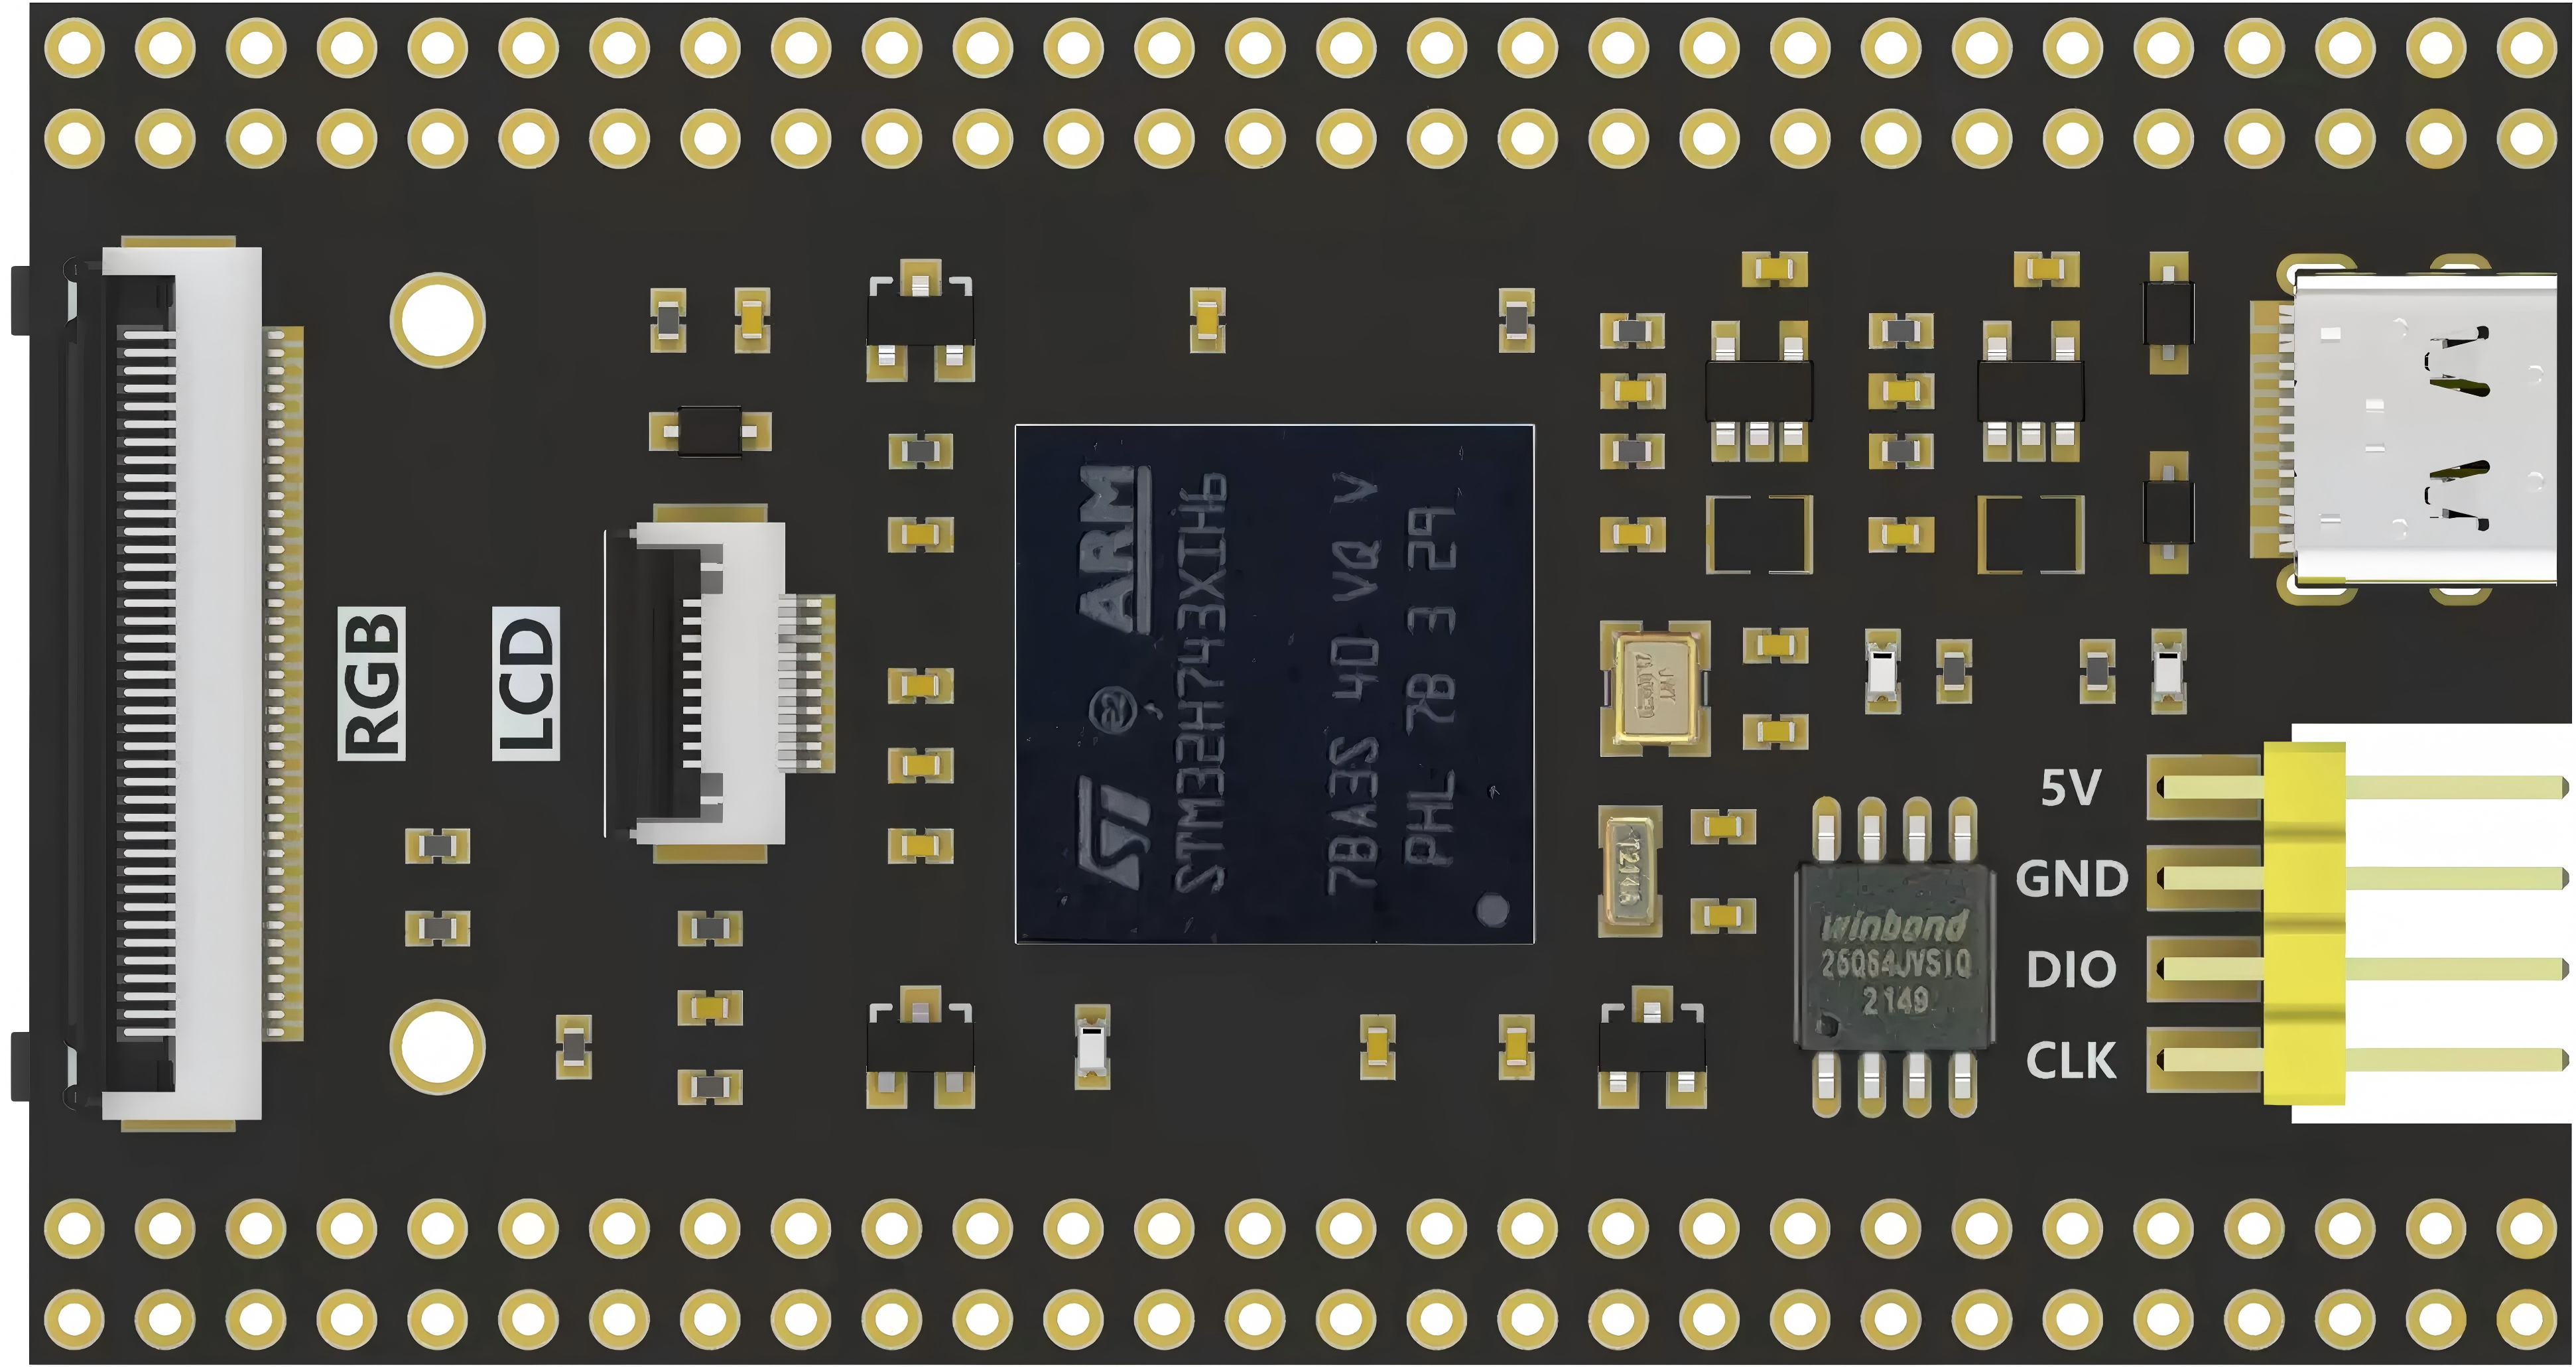
\includegraphics[width=0.55\textwidth]{images/chapters/fig-stm32h7-board.png}
\caption{STM32H743核心板实物图}
\label{fig:stm32h7-board}
\end{figure}

\section{IMU数据采集电路}

\subsection{IMU内部结构与工作模式}

系统选用HiPNUC六轴IMU传感器，内置三轴加速度计与三轴陀螺仪，通过片内算法完成姿态解算，可直接输出角速度、姿态角与加速度等物理量。该传感器采用UART接口与主控通信，默认波特率921600，输出频率可按需配置，典型工作模式下输出频率设置为100\,Hz以匹配控制周期要求。

通过合理配置量程与滤波参数，可在兼顾动态响应与噪声抑制的同时，为后续前馈补偿提供高质量数据。

\subsection{IMU时序与采样配置}

控制周期设置为10\,ms（对应采样频率100\,Hz），采用定时触发与DMA中断读取机制保证数据时序稳定。主控通过\texttt{hipnuc\_dec}模块对HiPNUC协议进行字节流解码：先执行帧同步与CRC校验，再按数据包类型提取角速度$\omega$、姿态角$\theta$与加速度数据。解析成功后数据被发布到控制路径，供IMU前馈补偿计算使用。

对于角速度小幅波动，工程采用死区处理策略，避免将传感噪声直接放大到执行端，提升闭环控制品质。

\FloatBarrier

\section{图像采集与通信电路}

\subsection{USB摄像头接入原理}

摄像头通过USB链路与上位机连接，形成图像采集与处理通道。该方案可降低主控侧图像处理压力，便于快速验证视觉算法。

为消除镜头几何畸变对PnP位姿解算的影响，需对摄像头进行标定。本文采用张正友棋盘格柔性标定方法\cite{Zhang2000calibration}，经棋盘格标定实验，所用摄像头的内参矩阵如式\eqref{eq:camera-matrix}所示：

\begin{equation}
\mathbf{K} = \begin{bmatrix} 435.37 & 0 & 318.68 \\ 0 & 433.86 & 226.72 \\ 0 & 0 & 1 \end{bmatrix}
\label{eq:camera-matrix}
\end{equation}

其中，$f_x{=}435.37$\,px、$f_y{=}433.86$\,px为焦距，$(c_x, c_y){=}(318.68, 226.72)$\,px为主点坐标。标定还同步获得径向畸变系数，标定后重投影误差可降至次像素级别，满足后续A4纸角点定位精度需求。

\subsection{图像数据链路设计}

图像链路设计关注带宽、延迟与稳定性，确保视频流在实验帧率下可持续传输，为实时跟踪与控制反馈提供数据支持。摄像头与linux主机通过USB 3.0接口连接，链路带宽可达5\,Gbps，远超720p@30\,FPS视频流的需求（约0.1\,Gbps），满足高带宽和低延时需求。同时使用屏蔽电缆线连接，提供更高的传输可靠性。

\FloatBarrier

\section{云台驱动与电机控制电路}

\subsection{电机驱动原理}

云台采用MS4010双通道电机驱动结构。偏航轴（Yaw）对应电机ID\,1，俯仰轴（Pitch）对应电机ID\,2，两轴通过RS485总线与主控通信，可实现位置模式与速度模式的在线切换，满足指向和跟踪两类控制需求。

系统上电后，主控扫描RS485总线发现ID\,1与ID\,2两台电机，完成云台初始化参数绑定、角度限位设置与回零动作，随后进入待命状态等待上层控制指令。MS4010 v3电机实物如图\ref{fig:ms4010-motor}所示，机身侧面的DIP拨码开关用于设定RS485设备地址（即电机ID），四位拨码对应二进制编码；底部印有RS485差分信号接线标识及电源正负极标注，安装时需严格核对极性以防驱动器损坏。

\begin{figure}[H]
\centering
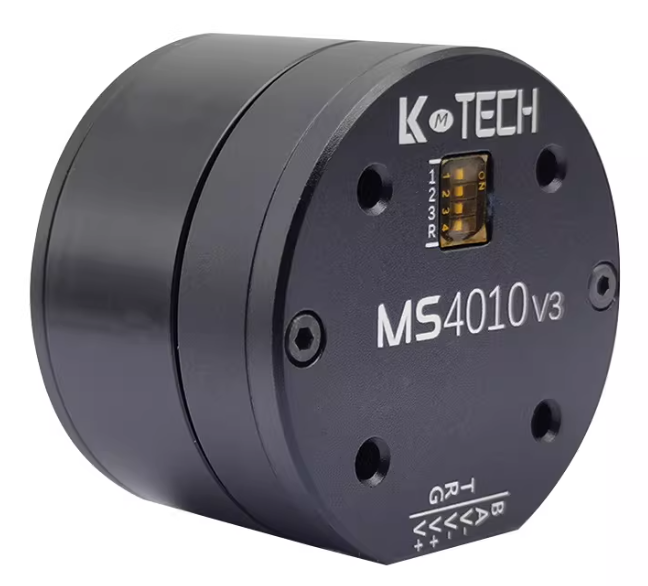
\includegraphics[width=0.8\textwidth]{images/chapters/fig-ms4010-motor.png}
\caption{MS4010 v3云台步进电机实物图}
\label{fig:ms4010-motor}
\end{figure}

\subsection{RS485总线接口与电源设计}

云台电机的控制信号经由UART外设驱动RS485收发器芯片后发出，MS4010电机以差分信号接收指令，并将编码器状态通过同一总线回报。设计中对供电冗余、地线回流与过流保护进行约束，总线终端匹配电阻置于链路末端，消除长线反射，提升整机稳定性。

系统采用12\,V锂电池统一供电，经TPS5400 DC-DC降压模块分别产生5\,V与3.3\,V轨为各子模块供电。电源电路原理图与PCB如图\ref{fig:power-schematic}和图\ref{fig:power-pcb}所示。

\begin{figure}[H]
\centering
\subfigure[电源电路原理图\label{fig:power-schematic}]{{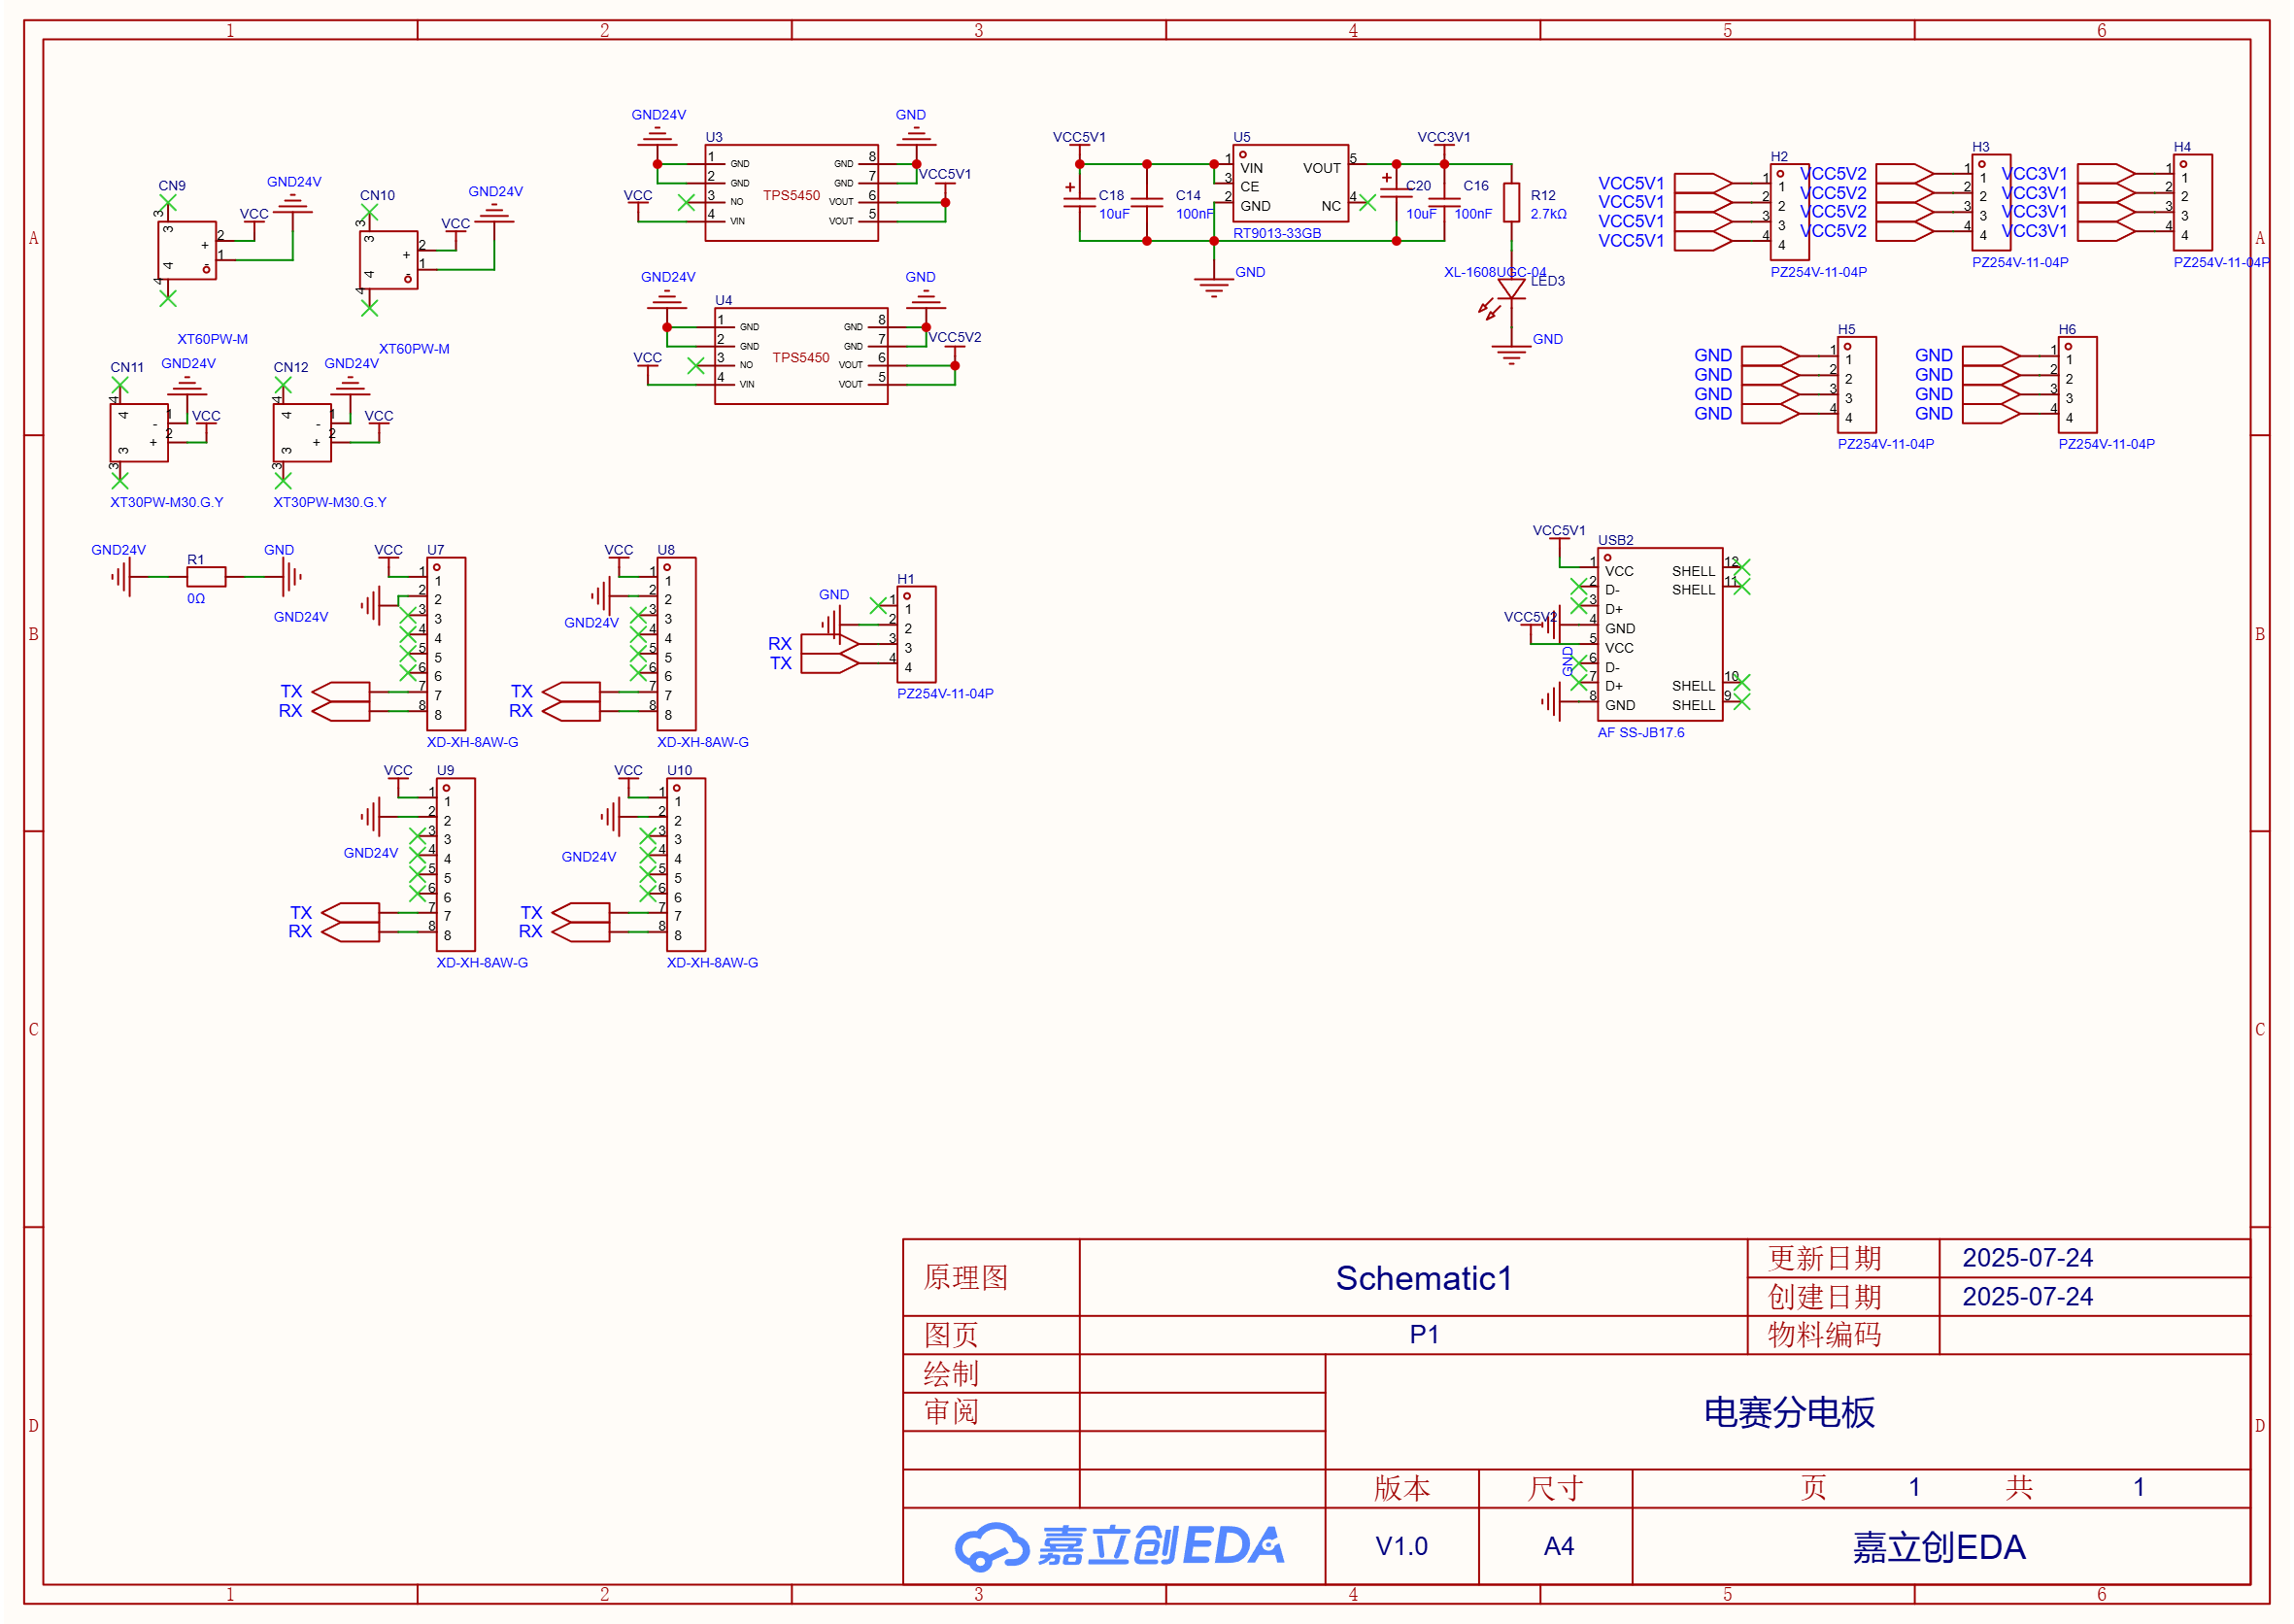
\includegraphics[width=0.7\textwidth]{images/chapters/fig-power-schematic.png}}}
\hfill
\subfigure[电源电路PCB布局\label{fig:power-pcb}]{{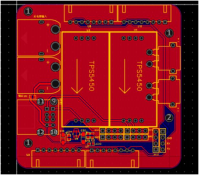
\includegraphics[width=0.7\textwidth]{images/chapters/fig-power-pcb.png}}}
\caption{电源电路原理图与PCB布局}
\label{fig:power-board}
\end{figure}

电源设计采用双路TPS5400降压芯片，保证各节点在满载条件下的供电稳定性；接线端子处增加滤波电容，抑制电机启停产生的电源纹波对信号链路的干扰。

\FloatBarrier

\section{自动循迹底盘控制电路}

底盘子系统以MSPM0G3507（Arm Cortex-M0+，80\,MHz）为主控，连接八路模拟量灰度传感器与MG513X减速电机编码器。相比数字量灰度传感器，模拟量传感器可输出连续电压信号，内置自动校准功能，无需每次重启重新标定阈值，更有利于差速Cloud PID控制的丝滑运行。底盘控制电路原理图与实物如图\ref{fig:chassis-schematic}和图\ref{fig:chassis-pcb}所示。

\begin{figure}[H]
\centering
\subfigure[自动循迹底盘电路原理图\label{fig:chassis-schematic}]{{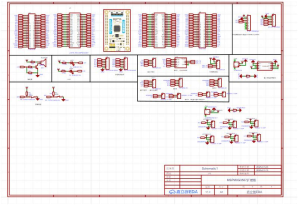
\includegraphics[width=0.6\textwidth]{images/chapters/fig-chassis-schematic.png}}}
\hfill
\subfigure[自动循迹底盘电路PCB实物图\label{fig:chassis-pcb}]{{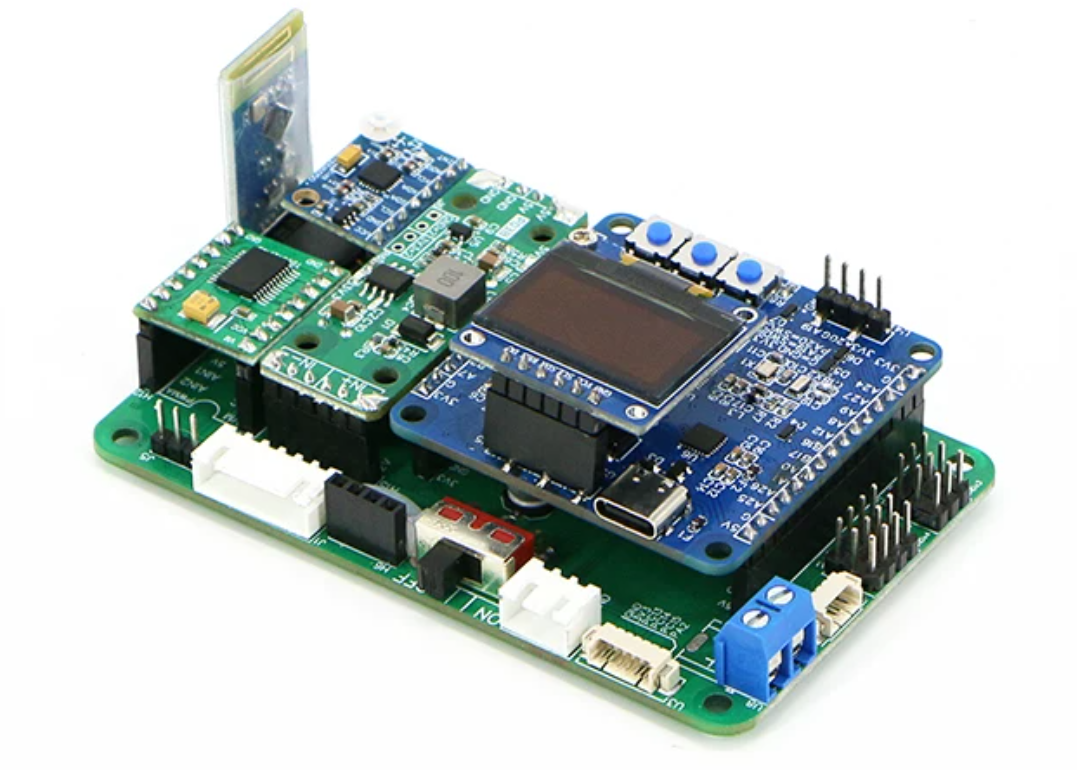
\includegraphics[width=0.6\textwidth]{images/chapters/fig-chassis-board.png}}}
\caption{自动循迹底盘电路原理图与PCB实物图}
\label{fig:chassis-board}
\end{figure}

底盘PCB集成了MSPM0G3507核心、电机驱动H桥电路、灰度传感器ADC接口与编码器采样电路；板载TPS5400为主控和传感器分别提供稳压；布局时将大电流电机驱动区与信号采集区隔开，降低电磁干扰。图\ref{fig:mspm0g-board}为WHEELTEC C07A底盘核心板实物图，核心芯片为MSPM0G3507，板上集成两颗用户按键可触发运行模式切换，电机驱动与灰度传感器接口通过排针引出，便于扩展与更换。

\begin{figure}[H]
\centering
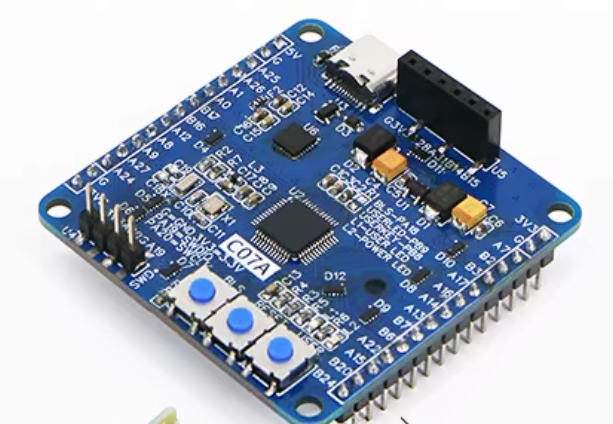
\includegraphics[width=0.55\textwidth]{images/chapters/fig-mspm0g-board.png}
\caption{WHEELTEC C07A底盘核心板（MSPM0G3507）实物图}
\label{fig:mspm0g-board}
\end{figure}

% \section{系统硬件联调与整机连接图}

% 在整机联调阶段，对模块连接、接口映射和供电路径进行一致性检查，形成完整硬件连接关系图，并验证系统基本功能可运行。

% 系统三个计算节点间的物理连接关系如下：Linux视觉节点（上位机）通过USB接摄像头完成图像采集，同时通过UART串口与STM32H7云台主控相连，发送目标像素数据；STM32H7主控通过UART接收HiPNUC IMU数据，通过RS485总线驱动MS4010双轴电机（偏航轴ID\,1、俯仰轴ID\,2）；底盘主控节点独立连接八路灰度传感器阵列与左右编码器，承担差速机动执行。整机供电采用统一电源总线，各节点自行管理本地去耦与保护，避免强电设备对信号回路的干扰。

\section{本章小结}

本章在总体架构与器件选型的基础上，详细给出主控最小系统、IMU采集电路、图像采集与接口、云台驱动及电源与抗干扰设计等硬件子模块的电路思路与实现要点，包含原理图、PCB布局与接口定义。通过对供电、去耦、信号隔离与总线终端匹配的工程化处理，提升了测量可靠性与执行稳定性，为后续软件联调、整机集成与实验验证提供了可复现的硬件基础。
